\chapter{Fonctionalités}
Nous détaillerons dans cette partie les différentes fonctionalités que propose l'outil. Des exemples illustrés et des \dots  
\section{Histogrammes}
Type de diagramme répendu, l'histogramme fait partie des diagrammes que LoCD peut générer. L'exmple ci-dessus illustre un résultat basique avec la configure par défaut de LoCD soit : 
\begin{itemize}
\item
Une unique couleur : bleu
\item
Absence de titre, sous titre et notes
\item
Représentation 2D
\end{itemize}
Pour changer cette configuration par défault, se référer au chapitre configuration% références !!!!!
\begin{figure}[htbp]
\centering
  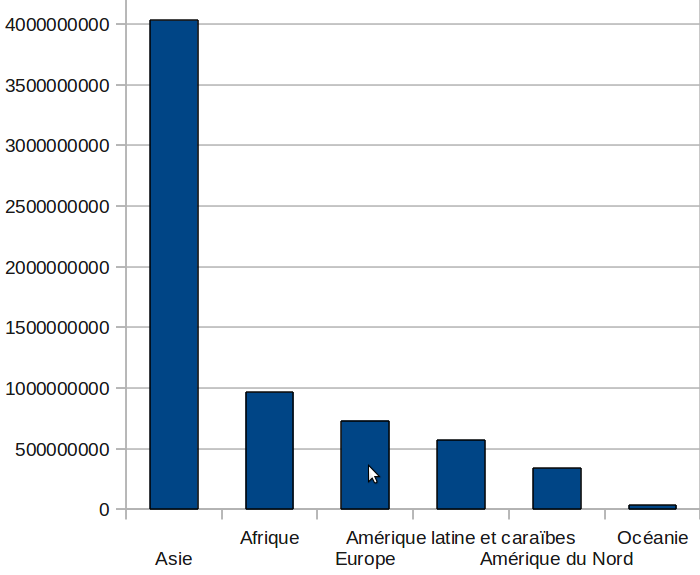
\includegraphics[scale=0.40]{img/diagrammebaton}
  \caption{Histogramme avec les paramètres par défaults}
  \label{fig:dbatons}
\end{figure}
  blah  blah  blah  blah  blah  blah  blah  blah  blah  blah  blah  blah  blah  blah  blah  blah  
\section{Diagrammes circulaires}
LoCD permet la création de diagrammes circulaires similaires  à celui présenté ci-dessous : 
\begin{figure}[htbp]
\centering
  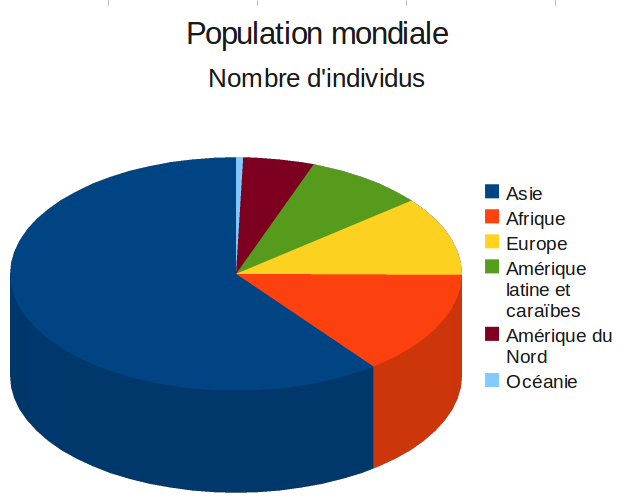
\includegraphics[scale=0.40]{img/diagrammecirculaire}
  \caption{Exemple avec un titre et un sous titre fournis dans les métas données.}
  \label{fig:dcirculaire}
\end{figure}

 blah  blah  blah  blah  blah  blah  blah  blah  blah  blah  blah  blah  blah  blah  blah  blah 

\section{Nuages de points}
\begin{figure}[htbp]
\centering
  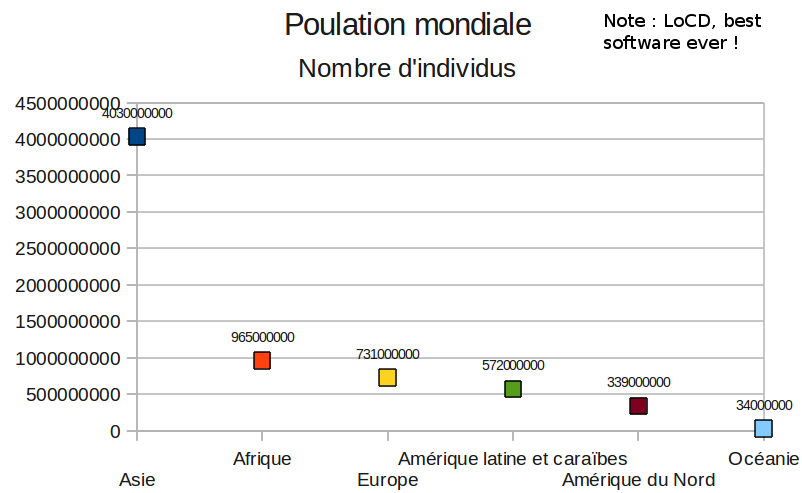
\includegraphics[scale=0.40]{img/diagrammenuages}
  \caption{Nuages de points avec toutes les méta données possible renseignées}
  \label{fig:dnuages}
\end{figure}  
  blah  blah  blah  blah  blah  blah  blah  blah  blah  blah  blah  blah  blah  blah  blah  blah 
  
